
\section{Introduction to vector fields on spheres} % <<<
\label{IntroductionToVectorFieldsOnSpheres}
\ifx\OutputIntroductionToVectorFieldsOnSpheres\undefined\else

We shall discuss some classical topics in homotopy theory.  A great deal of what we will cover owes much to the work of Frank Adams.  Today we look at a few of the problems (which turn out to have deep general significance), and begin with vector fields on spheres.  We define $S^{n-1} = \{x \in \R^n \mid \|x\| = 1\}$.  The idea is to assign to each point $x \in S^{n-1}$ a vector $v(x)$ tangent to $x$ in a smooth way, i.e., to find a map $v: S^{n-1} \to \R^n$ such that $v(x) \perp x$ for all $x \in S^{n-1}$.

\begin{wrapfigure}{r}{0.3\textwidth}
\centering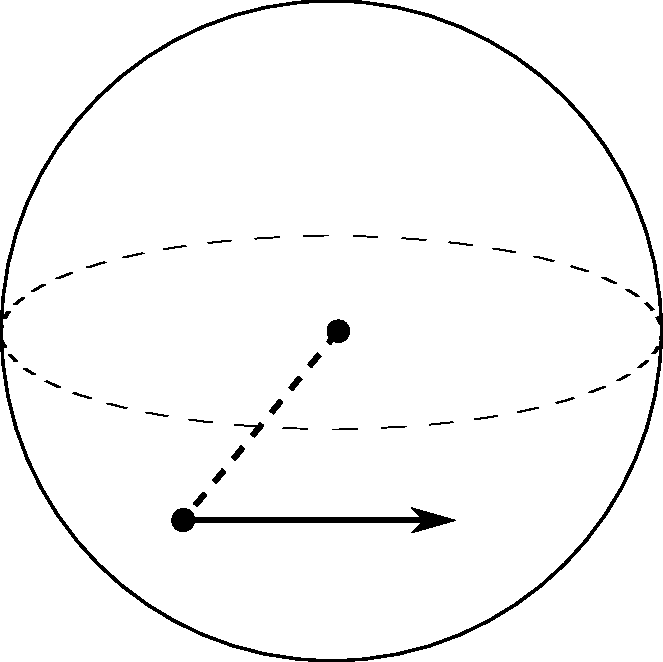
\includegraphics[width=0.2\textwidth]{figures/fig1.pdf}
\caption{\small Single point of a vector field. $x - 0$ is dashed, $v(x)$ is solid.}
\end{wrapfigure}

Now of course there's always the zero vector, which isn't very interesting, so in particular we'll look for nowhere-zero vector fields, which means we can normalize $\|v(x)\|$ to be 1 for all $x$, thereby giving a map $v: S^{n-1} \to S^{n-1}$ such that $v(x) \perp x$ for all $x \in S^{n-1}$. % everything is transverse to zero

Suppose that $n$ is even, so $n = 2k$ for some $k$.  Then $S^{n-1}$ can be thought of as $\{x \in \C^k \mid \|x\| = 1\}$, and $v(x) = ix$ works, so we have a nonvanishing vector field on all odd spheres.  However, when $n$ is odd, then there are none.  Such a $v(x)$ would give a homotopy between the identity and the antipodal map $\alpha(x) = -x$: \[h_t(x) = x \cos \pi t + v(x) \sin \pi t.\]  So $\deg \alpha = 1$.  But $\alpha$ is a composite of $n$ reflections in $\R^n$, so $\deg \alpha = (-1)^n = -1$, thus giving a contradiction.

\begin{wrapfigure}{r}{0.3\textwidth}
\centering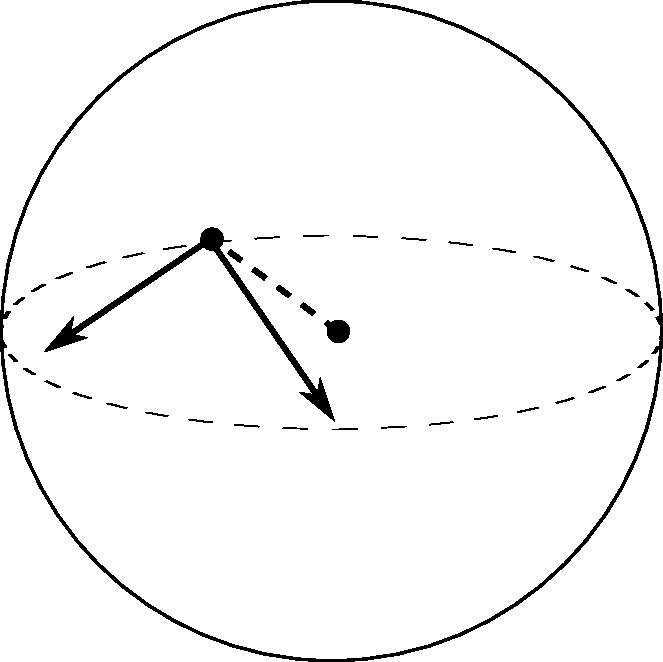
\includegraphics[width=0.2\textwidth]{figures/fig2.pdf}
\caption{\small An orthonormal $2$-frame at $x$.}
\end{wrapfigure}
Now the next question is how many linearly independent vector fields there are on $S^{n-1}$.  Using Gram-Schmidt we can reduce to the case that any set of linearly independent vector fields on the sphere form an orthonormal set at each point.  This is interesting in its own right; we shall see in the long run that this question is equivalent to some important problems in homotopy theory.  For the time being, the way we will think of this is in terms of
\begin{align*}
V_{n, k} & = \{\hbox{orthonormal $k$-frames in $\R^n$}\} \subset (S^{n-1})^k, \\
\pi: &\,\, V_{n, k} \to S^{n-1}, \hbox{the first projection}, \\
v: &\,\, S^{n-1} \to V_{n, k}\hbox{ a section of $\pi$, i.e.\ a vector field}.
\end{align*}
You can check that $\pi$ locally trivial and thus gives a fiber bundle, and $v$ is in these terms a section of this bundle.  So now the question has become: what is the largest $k$ for which this bundle has a section?

\begin{thm}[Hurwitz, Radon, Eckmann; Adams]
Write $n$ as $n = k \cdot 2^\nu$ for $k$ odd, and $\nu$ as $\nu = 4b + c$, $0 \le c \le 3$, and set $\rho(n) = 8b + 2^c$.  Then there exist $\rho(n) - 1$ independent vector fields on $S^{n-1}$ (Hurwitz-Radon-Eckmann) and no more (Adams).
\end{thm}
The first curious fact here is that $\rho$ depends only on the even part of $n$.
\[\begin{array}{c|cccccccc}
\nu & 0 & 1 & 2 & 3 & 4 & 5 & 6 & 7 \\
2^\nu & 1 & 2 & 4 & 8 & 16 & 32 & 64 & 128 \\
\hline
\rho(n) & 1 & 2 & 4 & 8 & 9 & 10 & 12 & 16
\end{array}\]
There are two steps to proving this:
\begin{enumerate} % should be participles
\item Construct them, which is fairly straightforward; we'll see that next session using Clifford algebras.
\item Show there are no more, which is much harder, and was the first major victory for $K$-theory.
\end{enumerate}
Before going on, now a corollary which in fact was known before this theorem was proved:
\begin{cor}[Kervaire, c.1956]
A sphere is said to be parallelizable when there is a basis for the tangent space, i.e., $\rho(n) = n$.  This occurs exactly when $n = 1$, $2$, $4$, or $8$, so the only spheres which have trivial tangent bundles are $S^0$, $S^1$, $S^3$, and $S^7$.
\end{cor}

A closely related problem is the so-called ``Hopf invariant 1 problem.''  Suppose $S^{n-1}$ is parallelizable, or equivalently that there is a section of $O(n) = V_{n, n} \to S^{n-1}$, called $v$.  Now a point in any ``Stiefel manifold'' $V_{n, k}$ can be written as a $(n \times k)$-matrix whose columns are orthogonal and have norm $1$.  The group $O(n)$ acts on $\R^n$ and this action induces an action on $S^{n-1}$.  Combining this with the section $v$ gives 
\begin{diagram}[height=2em]
O(n) \times S^{n-1} & \rTo & S^{n-1} \\
\uTo & \ruTo \\
S^{n-1} \times S^{n-1},
\end{diagram}
and $e_1$ is a right-unit of this multiplication on $S^{n-1}$, as $v$ is a section:
\begin{diagram}[height=2em]
(v(x), e_1) & \rMapsto & x \\
\uMapsto & \ruMapsto \\
(x, e_1).
\end{diagram}
Now $e_1$ isn't necessarily a left unit, but $v(e_1)$ is a matrix such that $v(e_1)_{i, j}$ is $1$ for $i = j = 0$ and $0$ whenever $i = 0$ or $j = 0$ but not both.  We can therefore correct the situation by replacing $v$ with $v(e_1)^{-1} v$, which will still be a section. % is this actually true?
Now $v(e_1) = I$, so we find that a parallelizable $(n-1)$-sphere has a multiplication with a $2$-sided unit.  Such a space is called an $H$-space; to be precise, an $H$-space is a pointed space $(X, x_0)$ with a product $\mu: X \times X \to X$ such that $\mu(x_0, x) = \mu(x, x_0) = x$.  In our cases, we have the correspondence
\[
\begin{array}{cccc}
S^0 & S^1 & S^3 & S^7 \\
\R & \C & \hbox{quaternions} & \hbox{``Cayley numbers''}.
\end{array}\]
In view of the results above, a natural question is: When can $S^{n-1}$ be given the structure of an $H$-space?

\ConfusedBox{
%\begin{wrapfigure}{r}{0.3\textwidth}
%\centering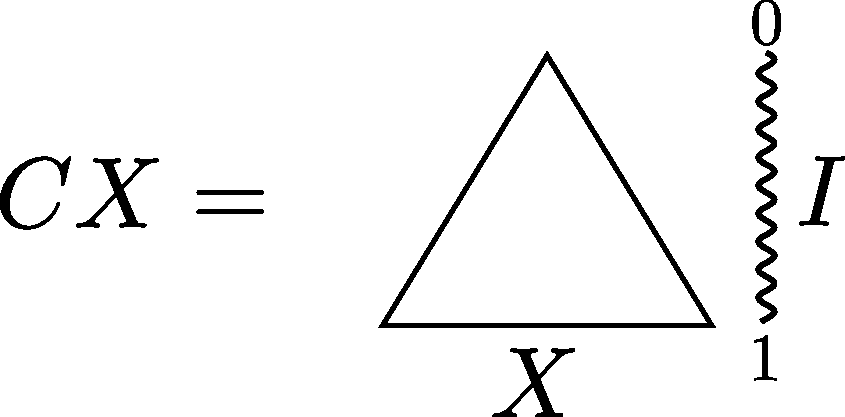
\includegraphics[width=0.2\textwidth]{figures/fig3.pdf}
%\caption{\small Diagram of the cone on $X$.}
%\end{wrapfigure}
\textbf{The Hopf construction is treated so much better in lecture \ref{TheMapsEandHinTheEHPLES}. I should really rewrite all this to reference that lecture.}

To attack this problem, it is helpful first to think about the map $\mu$ in ridiculous generality, sort of like thinking about a bilinear form in terms of a tensor product.  Namely, consider a map $\mu: X \times Y \to Z$, and consider the cone over $X$ which is defined to be the quotient $X \times I /\{(x, 0) \sim (x', 0)\}$.  The map $\mu$ then induces a map $CX \times Y \to CZ$ by $((x, t), y) \mapsto (\mu(x, y), t)$, and similarly a map $X \times CY \to CZ$.  $X \times Y$ includes into both $CX \times Y$ and $X \times CY$ as $((x, 1), y)$ and $(x, (y, 1))$ respectively, and $Z$ includes into $CZ$ as $(z, 1)$.  Putting these together, we get a diagram
%\begin{figure}[h!]
%\centering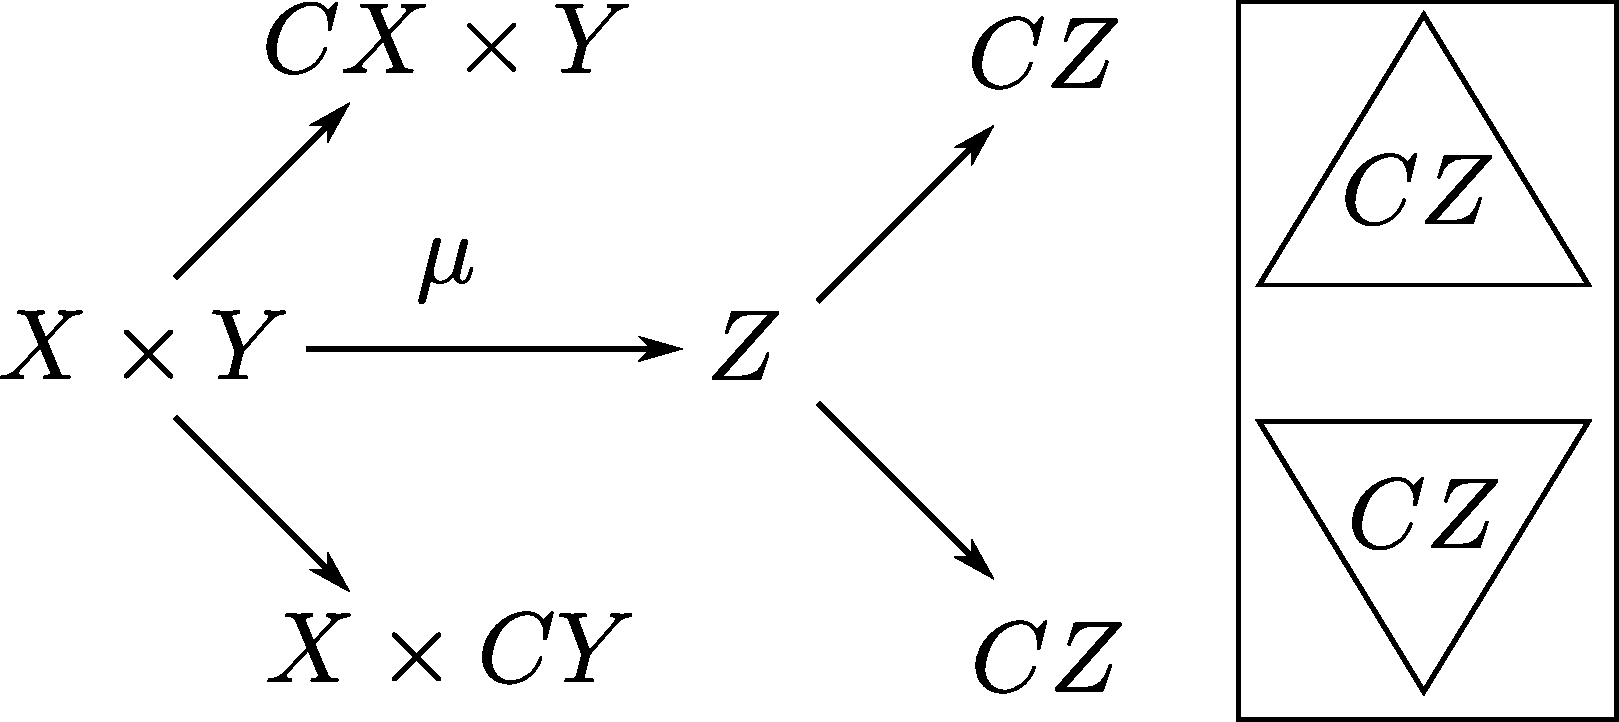
\includegraphics[width=0.35\textwidth]{figures/fig4.pdf} % %this guy is missing some arrows
%\end{figure}

The commutativity means that we can take the disjoint union of $CX \times Y$ and $X \times CY$ and identify along the copy of $X \times Y$ in each, then take two copies of $CZ$ and identify along their bases, and get a conglomerate map $H(\mu): X \ast Y \to \Suspend Z$, where $\ast$ denotes join and $\Suspend$ denotes suspension.
That is, the diagram above constitutes a map between two diagrams of shape $\bullet\leftarrow\bullet\rightarrow\bullet$, which induces a map $H(\mu)$ between their colimits (pushouts).
This process is called the ``Hopf construction'' for $\mu$, hence the name $H(\mu)$. 



We note two facts about the join: first, $S^{p-1} \ast S^{q-1} = S^{p + q - 1}$, which follows from the more general statement that $X \ast Y = \Suspend(X \sprod Y)$ for reasonable $X$ and $Y$, e.g., CW-complexes.  In the case of an $H$-space, $H(\mu)$ can be written as a map $X \ast X \to \Suspend X$, and if $X = S^{n-1}$, this is a map $S^{2n-1} \to S^n$, i.e., a homotopy class of a the $n$-sphere, something to be prized and studied. % use \pi_n notation here
}

\begin{wrapfigure}{r}{0.3\textwidth}
\centering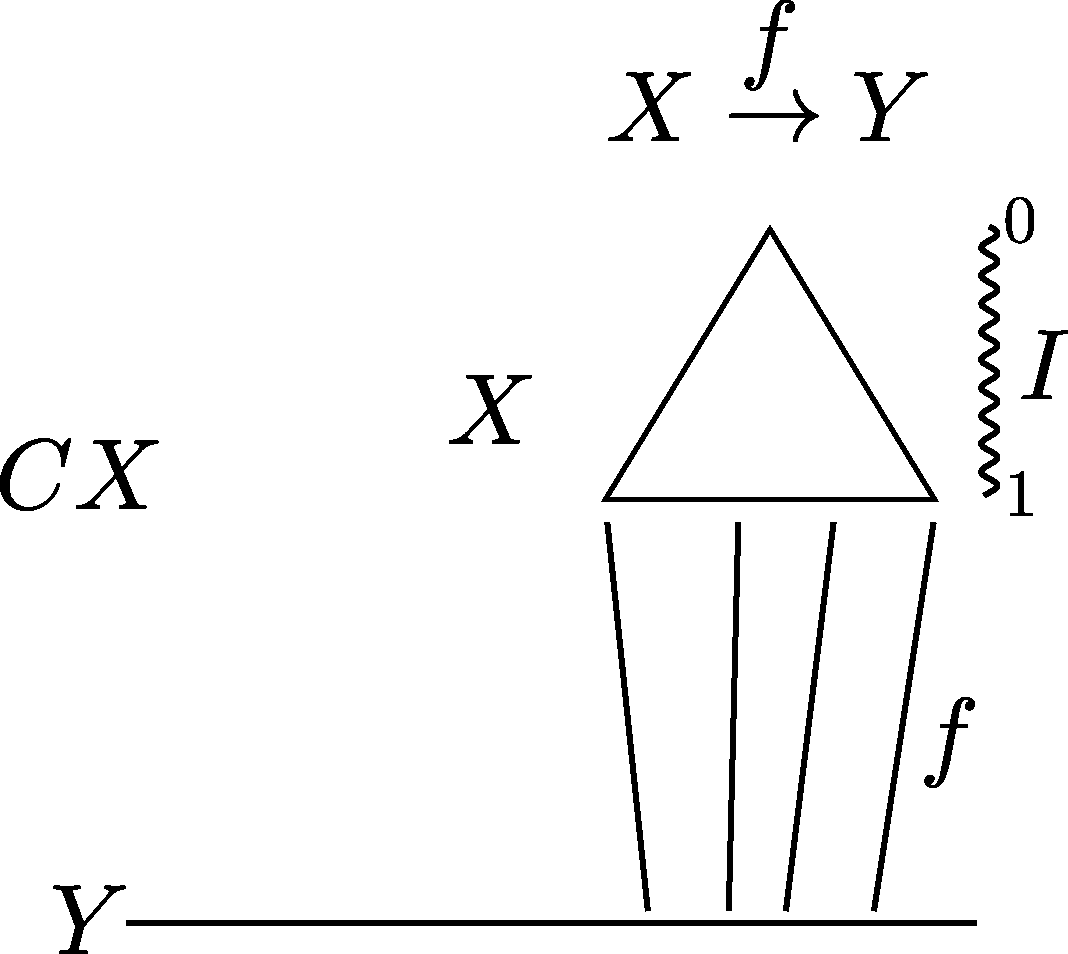
\includegraphics[width=0.23\textwidth]{figures/fig5.pdf}
\caption{\small Diagram of the mapping cone on $f$.}
\end{wrapfigure} % in the following paragraph, try to talk about the general case and the specific case of the cone on a Hopf map separately.  also, the definiiton of the cone is missing brackets and Y, CX change order.  'really means', 'is obstained by'
There is a duality in homotopy between maps and objects; namely, to every map there is an associated space which contains all the information about the map, called the mapping cone.  Associated to a map $f: X \to Y$, we build $C_f = Y \amalg CX / (x, 1) \sim f(x)$.  $Y$ includes into $C_f$ as its base, so one has a ``cofiber sequence'' $X \to Y \to C_f$.  Applying this to the map $H(\mu): S^{2n-1} \to S^n$, the mapping cone really means just attaching a $2n$-cell to $S^n$ via the map $H(\mu)$, so we get $S^{2n-1} \stackrel{H(\mu)}{\to} S^n  \to S^n \cup_{H(\mu)} e^{2n}$.  Now, (assuming $n > 1$) the cohomology is given by
\[
H^*(S^n \cup_{H(\mu)} e^{2n}) =
\begin{cases}
\Z & \hbox{generated by $y$ in degree $2n$,} \\
\Z & \hbox{generated by $x$ in degree $n$,} \\
\Z & \hbox{generated by $1$ in degree $0$.}
\end{cases}
\]
Using the cup product, $x^2 = \alpha y$ for some $\alpha \in \Z$, where for now $\alpha$ is well-defined only up to sign.  This coefficient $\alpha$ is called the Hopf invariant of $\mu$.  We make the unsubstantiated\footnote{Unsubstantiated for now --- see lecture \ref{TheMapsEandHinTheEHPLES}.} claim that $\alpha = \pm 1$ for $H(\mu)$ whenver $\mu$ is an $H$-space multiplication on the $(n-1)$-sphere.  As examples, we have
\begin{diagram}[height=2em]
S^3 & \rTo & S^2 & \rTo & S^2 \cup e^4 = \CP^2, \\
S^7 & \rTo & S^4 & \rTo & S^4 \cup e^8 = \mathbb{H}P^2, \\
S^{15} & \rTo & S^8 & \rTo & S^8 \cup e^{16} = \mathbb{O}P^2,
\end{diagram}
where the last is called the ``Cayley projective plane.''  (Note that nonassociativity of Cayley multiplication implies that there are no other Cayley projective spaces.) % what does this mean?  no higher OP^n, right?  not that there's anything after O...?

So now the question is: for what spheres is there an element of $\pi_{2n-1} S^n$ of Hopf invariant $1$?
\begin{thm}[Adams] % hopf invariant was only defined for n > 1 :)
If $\pi_{2n-1} (S^n)$ contains an element of Hopf invariant $1$, then $n = 1$, $2$, $4$, or $8$.
\end{thm}
For the time being, take a step back and recall the action $O(n) \times S^{n-1} \to S^{n-1}$.  Any $\alpha \in \pi_k (O(n))$ (not necessarily from a section) induces a map $S^k \times S^{n-1} \to O(n) \times S^{n-1} \to S^{n-1}$.  Doing the Hopf construction here induces a map $S^{k+n} \to S^n$, i.e., we get what turns out to be a homomorphism $J: \pi_k (O(n)) \to \pi_{n+k} (S^n)$ called the ``$J$-homomorphism.''  For $k < n$, $\pi_k (O(n))$ are known by Bott periodicity, hence there is much interest in the image of $J$.  Note that for $k < n$, $n + k > 2k$, and this is the so-called ``stable range'' where things often seem to work better; one then thinks of $J$ as a map $\pi_* (O) \to \Pi_*$.  The Adams conjectures are concerned with the image of this $J$. % should stablility really be mentioned here?

% >>>
\fi
\BoxedNote{\Bullet $S^{n-1}$ has $k-1$ linearly independent vector fields iff $V_{n,k}\downarrow S^{n-1}$ has a section.

\Bullet The largest $k$ such that there is such a section is $\rho(n)$, where we write $n=\textup{odd}\cdot 2^{\nu}$, $\nu=4b+c$ for $0\leq c\leq3$, and $\rho=8b+2^c$.

\Bullet The Hopf construction takes a map $\mu:X\times Y\to Z$ to a map $H(\mu):X*Y\to\Sigma Z$.

\Bullet If $S^{n-1}$ is parallelizable, it can be made into an H-space (essentially, apply the Hopf construction to a section $V_{n,n}\downarrow S^{n-1}$). This happens when $n=1,2,4,8$ by the previous point.

\Bullet (It is claimed that) if $\mu$ is an $H$-space multiplication on $S^{n-1}$, $H(\mu)$ has Hopf invariant one. We'll see later that this  can only happen when $n=1,2,4,8$.

\Bullet The $J$-homomorphism $J:\pi_k(O(n))\to \pi_{n+k}(S^n)$ sends $\alpha:S^k\to O(n)$ to the Hopf construction applied to $S^k\times S^{n-1}\xrightarrow{\alpha\times1}O(n)\times S^{n+1}\to S^{n-1}$.
}
\section{Clifford algebras} % <<<
\label{CliffordAlgebras}
\ifx\OutputCliffordAlgebras\undefined\else

In this lecture we will see how many vector fields on spheres we can construct using linear algebra; we will use Clifford algebras.  For more information, see for example the book by Strang.

For $k \ge 0$, the Clifford algebra $C_k$ is the associative $\R$-algebra generated by $e_1, \ldots, e_k$, subject to relations
\begin{align*}
e_i e_j + e_j e_i & = 0 \hbox{\;for $i \ne j$}, \\
e_i^2 & = -1.
\end{align*}
For example,
\begin{align*}
C_0 & = \R, \\
C_1 & \cong \C, \hbox{ note: you can identify $e_1$ with $i$ or $-i$, so the iso.\ is not canonical} \\
C_2 & \cong \mathbb{H}, \hbox{ with, say, $e_1 \mapsto i$, $e_2 \mapsto j$, $e_1 e_2 \mapsto k$}
\end{align*}
Note that the relations specify that we can give a basis for $C_k$ as the set of words $\{e_{i_1} \cdots e_{i_m} \mid m \ge 0, i_1 < \cdots < i_m\}$ made up of ordered nonrepeating sequences of the generators.  So $\dim C_k = 2^k$.  Note also that the collection $G_k = \{ \pm e_{i_1} \cdots e_{i_m} \mid m \ge 0, i_1 < \cdots < i_m\}$ is a multiplicative subgroup of $C_k$.  Also, $C_k$ comes equipped with an antiautomorphism $C_k \to C_k$, defined on generators by $\bar e_i = -e_i$, and extended to $C_k$ as an antiautomorphism.  It is an anti-involution in the sense that $\overline{xy} = \bar y \bar x$.

Before describing the $C_k$ further, let's look at how they can be used to construct vector fields on spheres.  One gets there by finding representations of $C_k$. Suppose $V$ is an $n$-dimensional vector space with a $C_k$-module structure $C_k \otimes_\R V \to V$.  $V$ is then a representation of $C_k$.  Next choose any inner product on $V$.  By averaging over the action of $G_k$ we can construct a $G_k$-invariant inner product $(-, -)$.  Let $S(V)$ denote the unit sphere of $V$, and note that points of $S(V)$ are invariant under action by the $e_i$.  We claim
\begin{thm}
For $x \in S(V)$, $\{e_1 x, \ldots, e_k x\}$ defines an orthonormal $k$-frame on $S(V) \cong S^{n-1}$.
\end{thm}
\begin{proof}
First, $(x, e_i x) = (e_i x, e_i e_i x) = -(e_i x, x) = -(x, e_i x)$, so $(x, e_i x) = 0$ and $e_i x$ is tangent to $S(V)$ at $x$.  Second, if $i \ne j$, we have $(e_i x, e_j x) = (e_i e_j e_i x, e_i e_j e_j x) = (-e_i^2 e_j x, e_i e_j^2 x) = (e_j x, (-e_i x)) = -(e_i x, e_j x)$.  So $(e_i x, e_j x) = 0$, and $e_i x$ and $e_j x$ are orthogonal.
\end{proof}
In particular, one way to find an orthonormal $k$-frame on $S^{n-1}$ is to find an $n$-dimensional $C_k$-module. To find as may orthonormal vector fields as possible of $S^{n-1}$ we should find the largest $k$ such that $C_k$ admits an $n$-dimensional module.
Thus we will search for low-dimensional representations of $C_k$.

From now on, write $C^+_k$ for $C_k$. As we identify more of the algebras $C^+_k$, we build up the following table. The column $C^+_k$ identifies the isomorphism type of $C^+_k$ in terms of better known $\R$-algebras. Here, if $A$ is an $\R$-algebra, $A(r)$ is used as a shorthand for the algebra of $r\times r$ matrices with entries in $A$. For each $k$, we write $a_k$ for the minimal dimension of a nonzero $C^+_k$-module (see lemma \ref{MinRepsOfAlgs}). Note that $\mathbb{H}^2$ acts on $\mathbb{H}\cong\R^4$ via $(a,b)c=ac\overline{b}$, and similarly, $\R(8)^2$ acts on $\R^8$ via $(M,N)v=MvN^\textup{tr}$. The last column will be identified later.
%Michael: Should say here `of a minimal C_k-module, as shown in lemma \ref{}....' or something
\[\begin{array}{c|ccccc} % this table might go better after the calculations.  most the definition of phi over to the right as a log of a_k.  use less ridiculous notation for matrix rings.  why are these the minimum dimensions of the representations??
k& C^+_k& a_k & \varphi_k = \log_2 a_k &C^-_k \\\hline
0 & \R & 1 & 0 & \R \\
1 & \C & 2 & 1 & \R^2 \\
2 & \mathbb{H} & 4 & 2 & \R(2) \\
3 & \mathbb{H}^2 & 4 & 2 & \C(2) \\
4 & \mathbb{H}(2) & 8 & 3 & \mathbb{H}(2) \\
5 & \C(4) & 8 & 3 & \mathbb{H}(2)^2 \\
6 & \R(8) & 8 & 3 & \mathbb{H}(4) \\
7 & \R(8)^2 & 8 & 3 & \C(8) \\
8 & \R(16) & 16 & 4 & \R(16).
\end{array}\] % the multiplication in the product of two algebras is component-wise -- wouldn't hurt to mention this
To identify the algebras $C_k^+$ it is useful to introduce a Clifford algebra associated to a different bilinear form. Let $C_k^-$ be the associative $\R$-algebra generated by $e_1, \ldots, e_k$, subject to relations $e_ie_j+e_je_i=0$ (for $i\neq j)$ and $e_i^2=1$. For the same reasons as $C_k$ (which from now on we call $C_k^+$), $C_k^-$ is $2^k$-dimensional.

  So what are the $C_k^-$?  $C_1^-$ has $1$ generator, whose square is $1$.  So $C_1^- \cong \R^2$, with $e_1 \mapsto (1, -1)$ (or $(-1, 1)$).  $C_2^- \cong \R(2)$ is the algebra of $(2 \times 2)$-matrices over $\R$.  The isomorphism is very noncanonical; try sending % awk
$e_1$ to reflection through $L_1$ and $e_2$ to reflection through $L_2$, where $L_1$ and $L_2$ are any lines separated by $45$ degrees.  Thus, $e_1e_2$ and $e_2e_1$ correspond to rotation by $90$ degrees, one clockwise and the other counterclockwise, depending upon the relative orientation of the lines.  This could get very tiring very quickly; fortunately that's as far as we need to go.  From now on, we use
\begin{lem}
For $k \ge 2$, $C_k^\pm \cong C_2^\pm \otimes C_{k-2}^\mp$.
\end{lem}
\begin{proof}
Again, this is highly noncanonical.  For example,
\[
e_i \mapsto
\begin{cases}
e_1 \otimes 1 & : i = 1, \\
e_2 \otimes 1 & : i = 2, \\
e_1e_2 \otimes e_{i-2} &: i > 2
\end{cases}
\]
works.  (As an exercise, complete this proof.)
\end{proof}

The remaining $C_k^\pm$ in the table can be computed in succession using this lemma, sort of like ``tying up the laces on a skate''; to do this one uses the following isomorphisms:
\begin{align*}
(\R \times \R) \otimes A & \cong A \times A \\
\R(n) \otimes A & \cong A(n) \\
\mathbb{H} \otimes \C & \cong \C(2) \\
\R(m) \otimes \R(n) & \cong \R(mn) \\
\mathbb{H} \otimes \mathbb{H} & \cong \R(4).
\end{align*}
From the table we can also quickly compute $C_k$ for $k > 8$ if we note the isomorphisms obtained by repeatedly applying the lemma:
\begin{align*}
C_k^+ & \cong C_2^+ \otimes C_{k-2}^- \\
& \cong C_2^+ \otimes C_2^- \otimes C^+_{k-4} \\
& \cong C_4^+ \otimes C_{k-4}^+ \\
& \cong C_4^+ \otimes (C_4^+ \otimes C_{k-8}^+) \cong C_8^+ \otimes C_{k-8}^+ \\
& \cong C_{k-8}^+(16).
\end{align*}
(Similarly, $C_k^- \cong C_{k-8}^-(16)$.)

The third column, $a_k$, corresponds to the minimal representation of the Clifford algebra $C_k^+$.  We can quickly determine this column using the following lemma:
\begin{lem}\label{MinRepsOfAlgs}
We compute the following dimensions of minimal representations of algebras:
\begin{enumerate}
\item When $A$ is a skew field, $A$ acting on itself is a minimal representation, so the minimal dimension is $1$.
\item When $A$ is a skew field and $A(n)$ is the space of $n \times n$-matrices over $A$, then $A(n)$ acting on $A^n$ is a minimal representation, so the minimal dimension is $n$.
\item When $A$ and $B$ are two algebras, then the dimension of a minimal representation for $A \otimes B$ is the minimum of the dimensions for minimal representations of $A$ and $B$ individually.
\end{enumerate}
\end{lem}
%Michael: Does this cover k=3,7
\begin{proof} These are easy exercises in commutative algebra. \end{proof}
The fourth column is $\varphi_k = \log_2 a_k$, where $a_k$ is the dimension of the minimal representation.  From $C_k^+ \cong C_{k-8}^+(16)$ we get that $a_{k+8} = 16 a_k$, or $\varphi_{k + 8} = \varphi_k + 4$.
% be consistent about whether phi should be a subscript or a function

Finally, we can apply this to vector fields on spheres.  There are $k$ linearly independent vector fields on $S^{a_k - 1}$; by taking $c$ copies of the vector space and using the diagonal action, there are $k$ linearly independent vector fields on $S^{ca_k - 1}$.  Now fix the dimension $n-1$ of the sphere and maximize $k$; i.e., for $S^{n-1}$, maximize $\{k\,:\,a_k | n\} = \{ k\,:\, \varphi_k \le \nu(n)\}$ (where $\nu(n)$ is the function from before).  The first few cases are:
\[\begin{array}{c|ccccccc}
\nu(n) & 0 & 1 & 2 & 3 & 4 & 5 & 6 \\
\hline
k_{max} & 0 & 1 & 3 & 7 & 8 & 9 & 11
\end{array}\]
and this is exactly $\rho(n) - 1$ from before.  So we have succeeded in constructing $\rho(n) - 1$ linearly independent vector fields on the $(n-1)$-sphere.  It turns out that this is the best we can do using linear algebra --- in fact this really is the best we can do with any tools.
\fi
\BoxedNote{
\Bullet We have constructed $k$ vector fields on $S^{n-1}$ whenever $a_k|n$, where $a_k=2^{\varphi_k}$ is the minimal dimension of a representation of $C_k$.

\Bullet We also noted that $a_k|n\iff k\leq\rho(n)-1$, and thus have constructed as many vector fields as possible.}

%>>>
